\setlength{\parindent}{10mm}

Tο \href{https://visualstudio.microsoft.com/downloads/}{\textbf{\uline{Visual Studio}}} είναι το IDE της Microsoft για το .NET για \textbf{Windows} και \textbf{Mac}.

\begin{enumerate}
    \item \textbf{Λήψη} Visual Studio από το Link παραπάνω.
    
    Επιλέξτε την έκδοση για το λογισμικό που σας ενδιαφέρει.
    \item Ανοίξτε το αρχείο .exe.

    \begin{figure*}[ht]
        \centering
        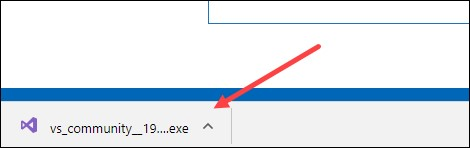
\includegraphics[scale=0.4]{images/inst1.jpg}
    \end{figure*}

    \item Στην επόμενη οθόνη, κάντε κλικ συνέχεια για να ξεκινήσετε την εγκατάσταση.

    \begin{figure*}[ht]
        \centering
        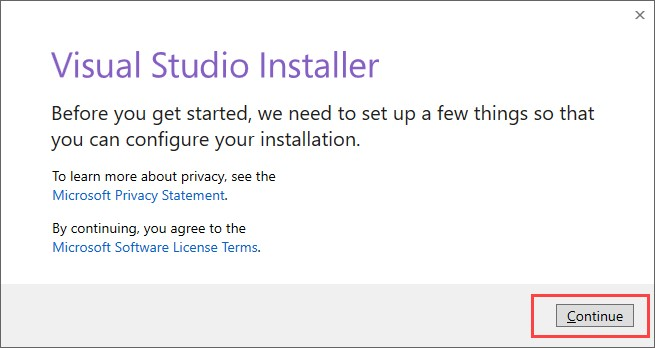
\includegraphics[scale=0.3]{images/inst2.jpg}
    \end{figure*}

    \item Αφήστε την εγκατάσταση να ολοκληρωθεί.

    \begin{figure*}[ht]
        \centering
        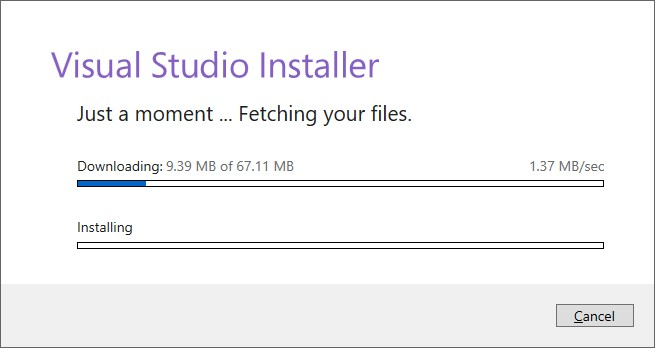
\includegraphics[scale=0.3]{images/inst3.jpg}
    \end{figure*}

    Visual Studio θα ξεκινήσει η λήψη των αρχικών αρχείων. Η ταχύτητα λήψης θα διαφέρει ανάλογα με τη σύνδεσή σας στο Διαδίκτυο.
    \\[4\baselineskip]
    \item Επιλέξτε την έκδοση λογισμικού που σας ενδιαφέρει.

    \begin{figure*}[ht]
        \centering
        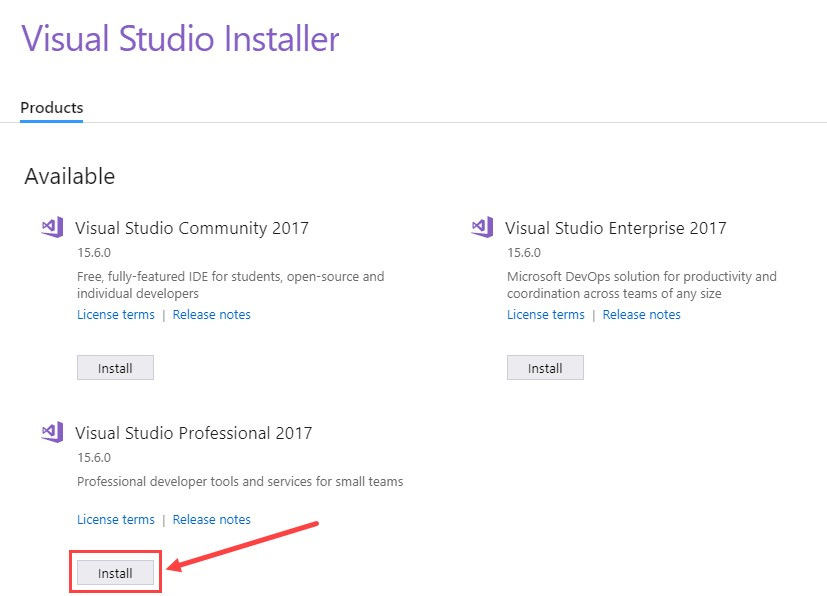
\includegraphics[scale=0.3]{images/inst4.jpg}
    \end{figure*}

    \item Επιλέξτε τα extensions που θα χρησιμοποιήσετε. Το .ΝΕΤ είναι επιτακτικό για C\#.

    \begin{figure*}[ht]
        \centering
        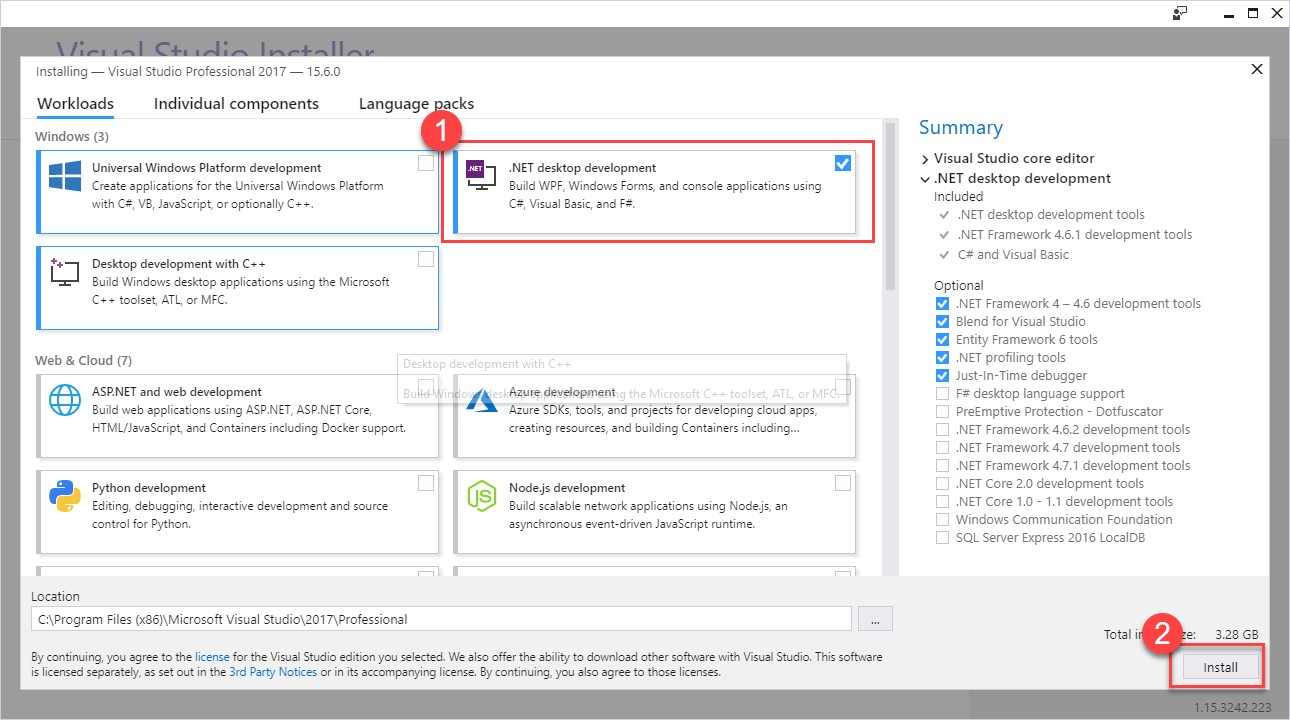
\includegraphics[scale=0.3]{images/inst5.jpg}
    \end{figure*}
    Πατήστε \textbf{Install} για να αρχίσει η εγκατάσταση.
    \\[8\baselineskip]
    
    \item Μόλις ολοκληρωθεί η εγκατάσταση των extensions χρειάζεται reboot.

    \begin{figure*}[ht]
        \centering
        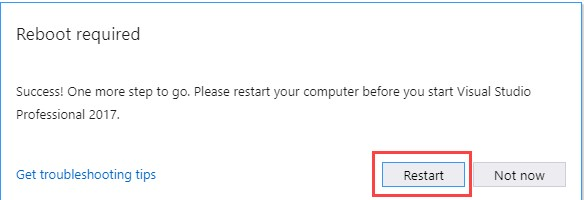
\includegraphics[scale=0.3]{images/inst7.jpg}
    \end{figure*}

    \item Ξεκινήστε την χρήση Visual Studio

    \begin{figure*}[ht]
        \centering
        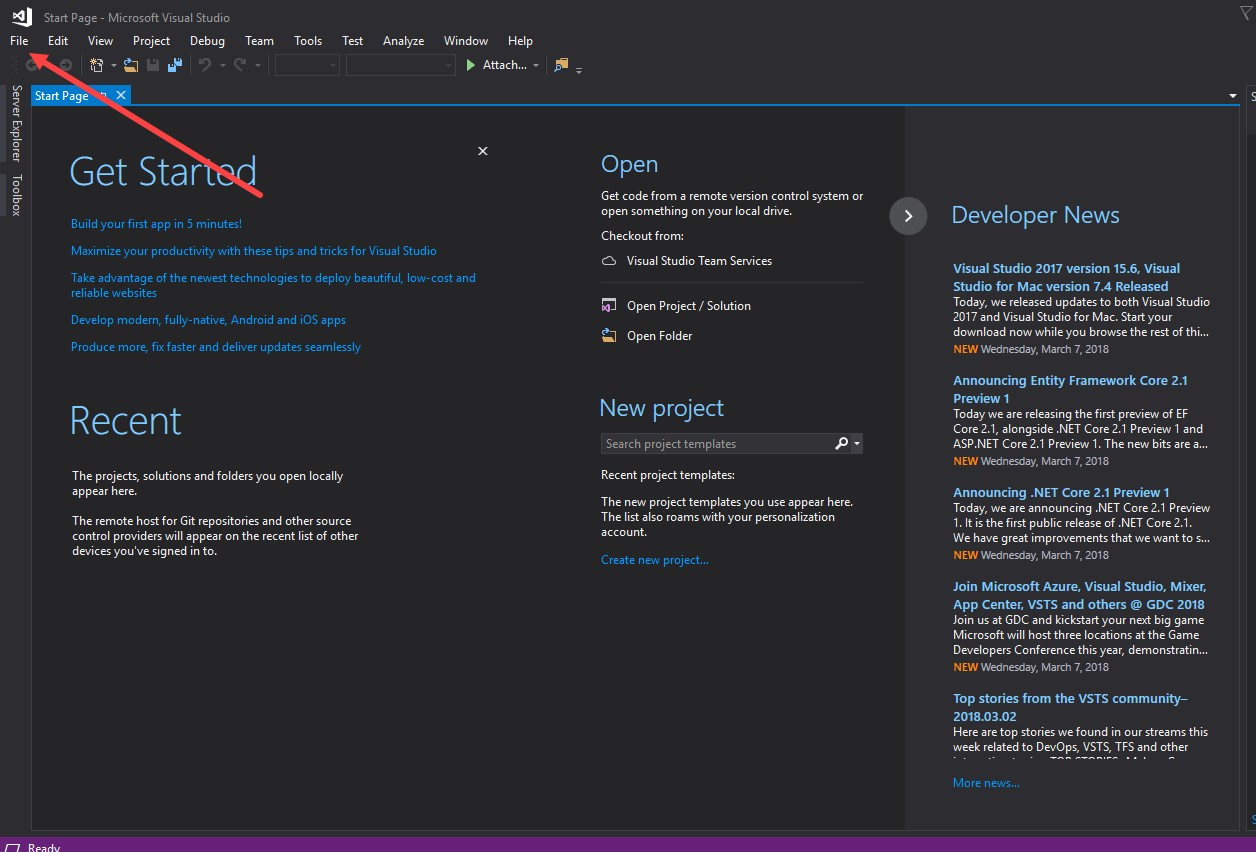
\includegraphics[scale=0.3]{images/inst8.jpg}
    \end{figure*}

    In Visual Studio IDE, μπορείτε να πλοηγηθείτε στο μενού \textbf{Αρχείο} για να δημιουργήσετε νέες εφαρμογές C\#.
\end{enumerate}

\textbf{Visual Studio Βασικά Xαρακτηριστικά.}

\begin{itemize}
    \item Δημιουργία μιας εφαρμογής σε οποιαδήποτε γλώσσα .Net.
    \item Δημιουργία οποιουδήποτε τύπου εφαρμογής.
    \item Εντοπισμός εφαρμογών εν κινήσει.
    \item Επεκτάσεις.
\end{itemize}
